%% This is a skeleton file demonstrating the use of IEEEtran.cls (requires IEEEtran.cls version 1.8a or later) with an IEEE conference paper.

%package list
\documentclass[conference]{IEEEtran}
\usepackage{cite}
\usepackage{graphicx}
\usepackage{hyperref}
\graphicspath{ {images/} }

\begin{document}

%Here goes the title

\title{CENG 435 Term Project Part-2 Group-26 Report}

%Authors List

\author
{\IEEEauthorblockN{\textbf{Sinan Talha KOSAR}}
\IEEEauthorblockA{Computer Engineering\\
Middle East Technical University\\
ANKARA\\
e2099190@ceng.metu.edu.tr}
\and
\IEEEauthorblockN{\textbf{FURKAN DOGAN}}
\IEEEauthorblockA{Computer Engineering\\
Middle East Technical University\\
ANKARA\\
e2098937@ceng.metu.edu.tr}
}
\maketitle


%Main body starts

\begin{abstract}
\label{abstract}
In the part 1 of this experiment we have already implemented TCP based connection between source and broker and UDP based connection for the rest. In this part, we created our own protocol on top of UDP to make UDP part reliable, that works on any topology or configuration network's. Our task is making UDP reliable for data transfer, although TCP is also provides us reliability. That's because RUDP is preferrable over TCP because TCP is not working properly (optimal) for network latency (the term used to specify any kind of delay that happens in data communication over a network). Sometimes, some properties of TCP is not desirable for building specific networks(e.g. game developers avoid TCP and make UDP reliable in the application level). In other words, in TCP, when any packet loss occurs, all subsequent of it are not allowed to occur in application-level until the lost one is re-transmitted(which causes another delay), even if they are still at other side of communication. To achieve this problems in some specific networks, RUDP is an option and in our experiment we have designed and implemented our RDT protocol on top of UDP.

\end{abstract}

\begin {keywords}
User Datagram Protocol(UDP), Transmission Control Protocol (TCP), Reliable Data Transfer(RDT), Reliable User Datagram Protocol (RUDP), Pipelining, Multi-homing, Routing Table, IPv4 addressing, Routing Mechanism, Socket Programming, UDP Sockets, Data Packets(Checksum, Header, Payload, Ack/nAck Mechanism, Sequence Number), Packet Loss Percentage, Corruption Percentage, Reordering Percentage
\end{keywords}

\section{Introduction}
\label{intro}
In this experiment, we have already had a basic topology. As stated in part $1$ of this experiment, there are $2$ different connection protocols(TCP \& UDP). In the first part, we have done this topology by writing scripts for each of the nodes[See part $1$ report]. In this part, the problem is unreliable network and our main goal is making this network reliable. Which we need to make only UDP part reliable, since TCP based connections are already reliable. The requested implementations are pipe-lining \& multihoming, which are methods for solve this problem, and remove the dependencies on routers' scripts. Briefly, we are asked to make unreliable part (UDP based connections) reliable, and implement specifications of our own protocol.
\newpage

\section{Design Part}
\label{section2}
In the second part of this experiment we are asked to design our protocol on top of UDP, and make it reliable, apply multihoming and pipe-lining. At the end, our protocol should be topology and configuration free which implies that our protocol should be applicable on any network designed by anyone with any configurations.
\subsection{Routing Table}
In the second part of term project we are asked to resolve dependencies on router's scripts, i.e. we need to modify routing tables to achieve this. By doing so, there is no need to write scripts for routers. The router nodes only responsible for routing data to appropriate IPs. Briefly, we can say that routing table has similar idea with mapping in package delivery. While sending data from one node to another, sender node must know where to send the data firstly. If there are no links connecting directly sender and receiver nodes, data must be send via other nodes using route tables in the way to find proper way. A node sends an IP packet to proper gateway in network then router decide how to route correct destination and gateways use routing table to keep track of data. Basically, routing table is a database to keep track of data like having a map to decide which way to forward in the traffic. When we have created a slice in \href{https://portal.geni.net}{GENI} platform for term project part 2 and added updated resources given in first part. After that default interfaces' IPs are shown ($Fig. 4$)[See Appendix in Section \ref{appendix}]\\
Based on $Figure 4$, the default routing table in routers are shown in $Fig. 5$ [See Appendix in Section \ref{appendix}]\\
In $Fig.5$ routing table shows if incoming packet destination matches with the IP in Destination column, then direct it to it's corresponding Gateway value. For example, if incoming packet's IP is $10.10.3.0$ in broker node, direct it to $10.10.2.2$, same situation is valid for other nodes. At this point we need to modify the routing table to remove the dependency on router's script. By writing route commands in machine, we have done that (To see all exact commands please check README.md)

e.g. sudo route add -net [IP of node that packet is destinated] netmask [Netmask] gw [IP of node to be routed] dev [link]\\
\newpage
After making modifications, route table for router 1 does:\\
Incoming packets having IP $10.10.3.0$ will be directed to $10.10.3.2$ and Ack/nAck packets having $10.10.2.0$ IP will be directed to $10.10.2.1$. For all other nodes same logic apply for them. See $Fig. 6$ [See Appendix in Section \ref{appendix}]\\
In the route table there are some $.0$ s in the IPs (e.g. $10.10.3.0$), it means in the place of $0s$, any value is accepted. More generally, in the design of servers, $0.0.0.0$ corresponds "all $IPv4$ addresses on the machine. 
\subsection{Main Design}
We have decided to use $python3$ to write scripts and create classes for each Source, Broker and Destination nodes. Sockets are opening with port numbers and IPs are assigned in constructors for all classes in our design. In source class we have created TCP connection and read the given large file as chunks which are $996$ $(MAX\_PACKET\_SIZE - 4)$ bytes (MAX\_PACKET\_SIZE depends on designer of applying topology) bytes for each, since we are adding headers to packets in broker node (default size $1000$ bytes). Since we are going to examine the time difference again (similar to part $1$), we got the time from \href{https://developers.google.com/time/}{NTP Server of Google} when first packet sent from source node and last packet received at destination to synchronization of the nodes. In broker, we have created $2$ classes, one for receiving data from source node and one for sending data to destination node. While receiving from source node only TCP rules apply (see part $1$ for detailed explanation) and as soon as packet received in receiver class, it pass that packet to sender class.We have realize that last packet that is sending with TCP is empty (b'') on broker node. Therefore, we used flags (basic integer variables to decide different situations -to be explained in corresponding sections-). When we read last packet from source node (which is empty(b'') because of TCP), we set flag variable to $2$ which we use as condition code to say it's the last packet that is going to be received and last packet it is going to be send. We need to apply multihoming which connects broker to destination with more than one routers. This provide us to increase performance. After doing so, broker decides that one packet is forwarding to destination from router $1$, other from router $2$. While $1$ packet is forwarding to router $1$, other needs to be forwarded to router $2$, to achieve this, we used threads in broker node. We need to create packets and parse packets in broker, while parsing we are parsing packet and calculate the necessary info from them. While making packet, we are creating packet and including necessary info in it. To validate the receiving packet, we make checksum comparison with checksum value in the packet and re-calculated rsum value from data in the packet. We have added cumulative ACKs for all window-sized packets instead of taking ACK for each of packet inorder to save time. When we send a packet in broker we have started a timer to determine timeouts (value is given $0.2$). To achieve the problem which if there are still unacked packets greater than window size or, packet is the last packet that we need to send while there are still unacked packets; we are waiting for correct acks without time-out. If there is no time-out, we set our variables to use them again, but if the packet is the last one, we send it again. When there is time-out, without making any modification, the reliability is breaking down. Therefore, we have applied reliable data transfer method, pipe-lining, in specific Go-Back-N. (Above paragraph is kind of description of Go-Back-N). In destination node's script, although our implementation is based on Go-Back- N, we are receiving packets unsorted order in some cases since we have applied multihoming in our network (receiving both from router $1$ and router $2$). So, just to be sure in order to sort packets and merge them correctly, first we are saving all packets in a list which is holding data then sort them. After receiving a packet, again we parse the packet, get the checksum value and sequence number in packet and calculate rsum value then compare them. If they match, we are sending ACK for next sequence number. If not, we are sending nAck for that sequence number. In Ack and nAck packets, we have checksum, flag, sequence number and empty data, since we are using them only for validation. When the last packet arrives, destination class get time from same NTP Server and print arrival time. If there is no traffic in between $60$ seconds, our destination timed-out. After receiving last packet correctly, we are writing our data, in the list that we have store them unsorted order, in sorting order. While sorting, python3 has sort() function which is called Tim Sort also, takes $O(n log n)$(This is one of the advantage that make us to decide to use python3 to write scripts). After making successful sorting we write our received packets to file $(output2.txt)$ respectively.

\section{Implementation Part}
\label{section3}
\subsection{Common Parts for All Nodes}
Since we are asked to design our own protocol that should be reusable for any topology or any network configuration based bandwidth, delay, and packet size, we are passing necessary inputs (IPs, port numbers and input file) while executing the scripts. How to done that will be explained in corresponding sub-sections of nodes. We have taken ordinary care while writing all of our functions in try catch block to detect any error in our code easily, which we might faced with while implementing the protocol and beyond that. Note that below sub-sections are methodology to overview of our codes. Mechanisms use to provide reliability are checksum, Ack/nAck, retransmission and sequence number. How this mechanisms work described in below-subsections. 
\newpage
\subsection{Source Node}
We pass IP address, and port number of broker and input file that is going to be sent over network as argument while executing the script, then in the code we are placing them in necessary places. To see how to execute $source.py$ file please check $README.md$.
In the requirements ,we are given maximum packet size as $1000$  bytes. Our readFile() function is reading the data as $996$ $(MAX\_PACKET\_SIZE - 4)$ bytes (MAX\_PACKET\_SIZE depends on designer of applying topology) since header will be added in broker. As soon as the sendFile() function starts, we are getting time from \href{https://developers.google.com/time/}{NTP Server of Google} to synchronization of the nodes and write the time to time.txt file(just for working on local machine). We are not going to send time in the packet since in this part of this experiment is not focusing on delays. Therefore, the time that written first at time.txt is the time of first packets' sending time to broker. In source node we create TCP connection as: 

self.localSocket = socket.socket(socket.AF\_INET,\\
socket.SOCK\_STREAM)\\
where AF\_INET is for IPV4, and SOCK\_STREAM is for TCP. \\
Since in this experiment we need to construct a network to reliable data transfer, we don't need to apply any protocol that is written by us to TCP part. Basically, we are reading input packet by packet and sending to broker packet by packet in TCP part.\\
\subsection{Broker Node}
We are passing port number of source, router $1$'s IP and port number and router $2$'s IP and port number as argument, since we are going to implement multihoming to make the transaction faster, broker should know where to send which means routers' IP addresses and port numbers. Then in the code we are placing them in necessary places. To see how to execute $broker.py$ file please check $README.md$. In broker basically we are doing 3 operations:

Receiving packet from source

Forming actual packets(packet form for reliable data transfer)

And sending it to destination via appropriate router\\
While receiving packet we need to open appropriate socket connection with source node (TCP connection), with:

self.localSocket = socket.socket(socket.AF\_INET,\\
socket.SOCK\_STREAM)\\
After creating successful connection between source, broker is accepting the packets in recv() function. As soon as the recv() function called, it construct the object which sends packets to destination with sender's window size and set time-out (depends on RTT of applying topology) value for receiver socket, and after, we are writing that packets to $output.txt$ just for manually check the transmission is successful. Since we are sending $996$ $(MAX\_PACKET\_SIZE - 4)$ bytes (MAX\_PACKET\_SIZE depends on designer of applying topology) bytes from source, naturally we are accepting the packets in same length. We have used flags(basic integer variables) in our protocol design to check the conditions in the code flow. In the broker, the flag values are:

flag = $0$ is for first packet

flag = $1$ is for rest of the packets

flag = $2$ is for last packet\\
Based on the flag values, we can track the packets basically. We have implemented multihoming in broker. So, broker picks one of the router and send the packet to destination across to that router. To make decision we get a random value between $0$ and $1$. And if the random number is in interval $[0,0.5)$, broker picks router $1$, and if random number is in interval $[0.5, 1]$, broker picks other router. As stated in Common Parts for All Nodes sub-section, we need to design a protocol that should be reusable for any given topology or configuration, that's why we have implemented the decision of routers by getting random variable. In the future, if someone decides to change the number of routers, the modification can be done easily by changing the interval for routers. After picking router to send via, we start a thread for it, because our protocol is pipe-lined, i.e. to send another packet, our program won't wait to finish current packet sending process. After starting threads, we have joined them so, main thread will wait our threads to finish their job before halting the program. Each thread is working same but with different parameters. Below implementation of SendToDest class' is similar for each threads. While sending SendToDest class has send() function. When a packet arrives to broker from source the process for send() starts (it is not waiting all packets for arrive to broker from source since the connection between source and broker nodes are TCP based, there won't be any package loss). In that process, broker mark all received packets as unacked and form packet according to checksum, sequence number, flag and data values in makePacket() function. Packet consists given sequence number as $2$ byte, checksum as $1$ byte, flag as $1$ byte, and the rest is our data. We calculate the checksum value by taking bitwise-and value of sum of our data and $0xff$ to get unsigned value, to avoid errors  arising from negative checksum values. In makePacket() function, we are converting the values to bytes and since we are going to design a topology or configuration independent protocol, we have indicated the byte values as 'little'. Because the machines that is going to implement our protocol may have different encoding like big-endian, so to make this encoding same for any machine we have stated byte-order as little-endian. After we have implemented our reliable data transfer method to our protocol, Go-Back-N. Our program waits ACK for unacked packets and check if unacked packets' count is greater than the window size or current packet is the last packet or there is still unacked packets that is waiting to be Acked, if so receive Ack from destination, after that if time-out occurs, it goes back N, prints "Go-Back-N"(just for visiualization for us indicating that Go-Back-N mechanism works) and send all N packets again with sendAll() function which sends all packets given. If not, it parses the packets with parsePacket() function, which parse packets contents and calculate new checksum from contents as receivedSum and returns. After that if checksums match we are setting a cumulative Ack number and remove them from unacked list, which increase our protocols' performance since process cumulative Acked packets instead of processing each packet. Then we have arranged the unAcked and lastAcked variables accordingly. While sending packet to destination, sendPacket() function works, sending packet to destination and adjust nextSequnceNumber then starting time-out value (depends on RTT of applying topology) for it's purpose. After all packets are received from source and transmitted to destination we closes the connection but since we are using threads, we separated the connection closing in a function to avoid main thread to close connection while other threads still in progress or even reading data.
\subsection{Destination Node}
In destination class, we also have $2$ threads for multihoming. We have ACK and NACK variables to see the counts of Acks and nAcks. When we receive packet in destination node, we parse the packet and to validate, compare the checksum with calculated checksum (rsum) and sequence numbers. Same properties apply for functions makePacket() and parsePacket() in broker node. When checksum or sequenceNumber checks fail, we create an nAck packet for erroneous packet and send it back, otherwise we send Ack packet and adjust sequence number. In destination class, when last packet arrived, we get the time from \href{https://developers.google.com/time/}{NTP Server of Google} again to synchronization of the nodes and save the time. After that same closing procedure as in broker applies to shutting down the connection. Note that, the packets for Acks and nAcks have sequence number as $2$ bytes, checksum as $1$ byte, flag as $1$ byte and the rest is our empty data.
\newpage


\section{Experiment Part}
\label{section4}
All results calculated with $95\%$ confidence-interval and margin of error for each of them less than $2.5\%$. We have used tool to calculate $95\%$ confidence interval from
\href{https://www.mathsisfun.com/data/confidence-interval-calculator.html}{$Confidence\_Interval\_Calculator$}
\subsection{Experiment I}
\begin{figure}[ht]
   \centering
   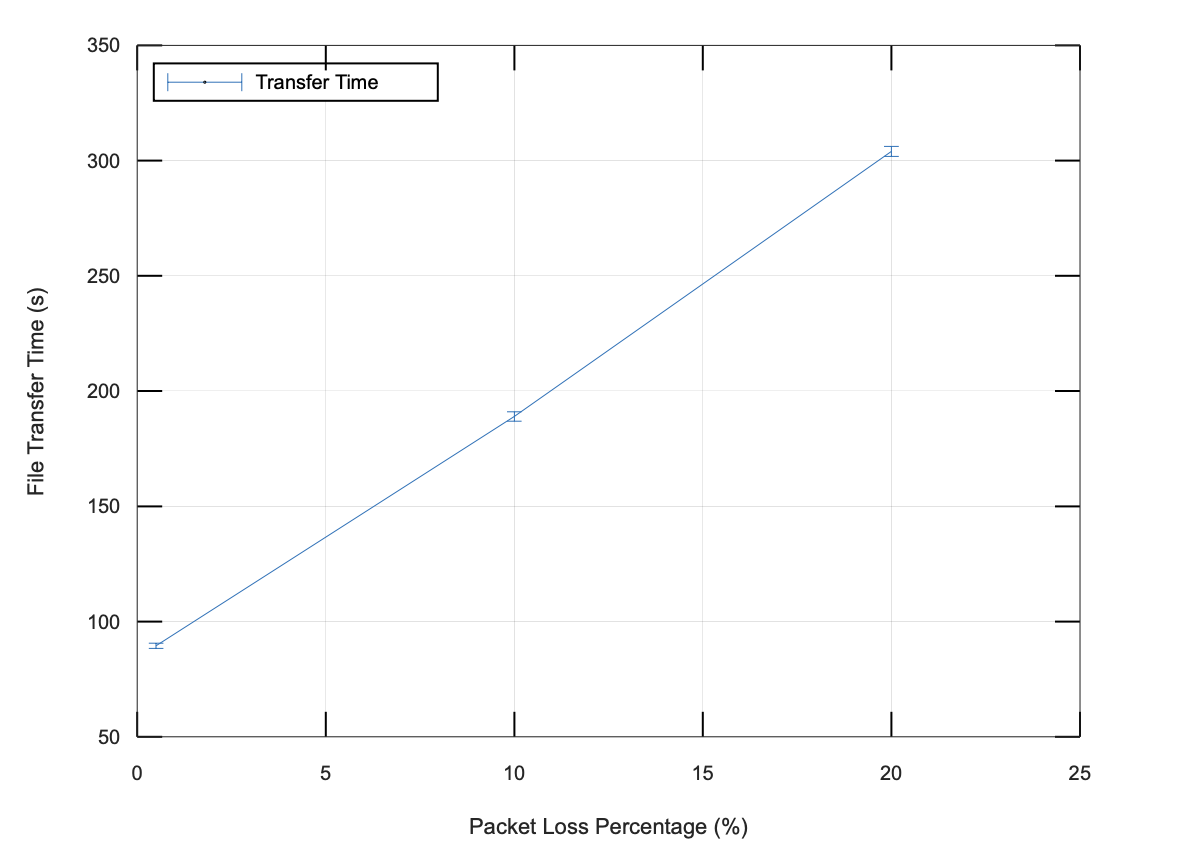
\includegraphics[scale=.45]{images/exp1.png}
    \caption{File Transfer Time(s) vs Packet Loss Percentage(\%)}
    \label{fig:topology}
\end{figure}
The confidence intervals are :

$89.5 \pm 1.12$

$189 \pm 2.04$

$304 \pm 2.16$\\
Our protocol is reliable, so when packet loss occurs, re-transmission starts with Go-Back-N, then sent lost packets again. As we can see from the Figure 1, when packet loss percentage increased, file transfer time also increased because there were more re-transmitted packets. As a result, we have observed that packet loss percentage and file transfer time is directly proportional to each other.
\newpage
\subsection{Experiment II}
\begin{figure}[ht]
   \centering
   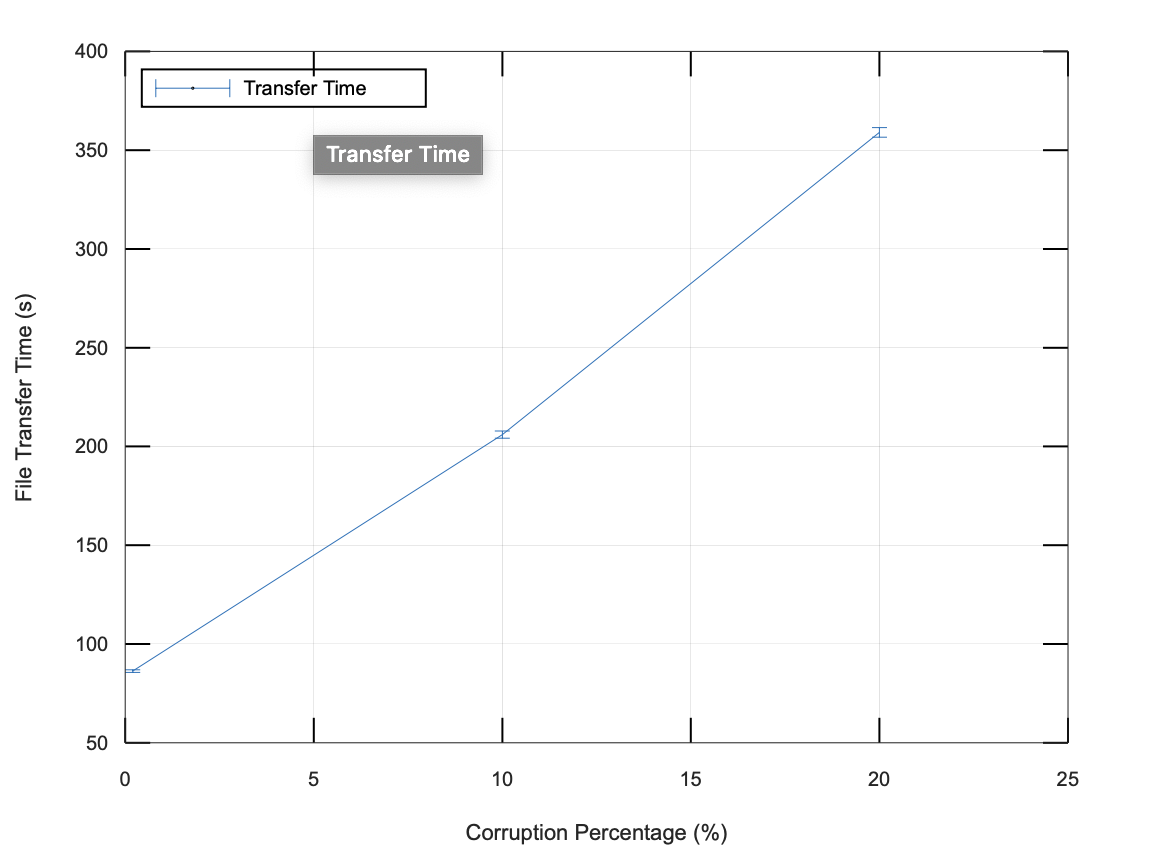
\includegraphics[scale=.45]{images/exp2.png}
    \caption{File Transfer Time(s) vs Corruption Percentage(\%)}
    \label{fig:topology}
\end{figure}
The confidence intervals are :

$86.3 \pm 0.627$

$206 \pm 1.8$

$359 \pm 2.42$\\
We used mechanisms use to provide reliability, one of them is checksum. When checksum value in the header and re-calculated checksum value doesn't match, it means that there is corruption in packets. When corrupted data received at destination, re-transmission starts with Go-Back-N, then sent corrupted packets again. As we can see from the Figure 2, when corruption percentage increased, file transfer time also increased because there were more re-transmitted packets. As a result, we have observed that corruption percentage and file transfer time is proportional to each other.
\subsection{Experiment III}
\begin{figure}[ht]
   \centering
   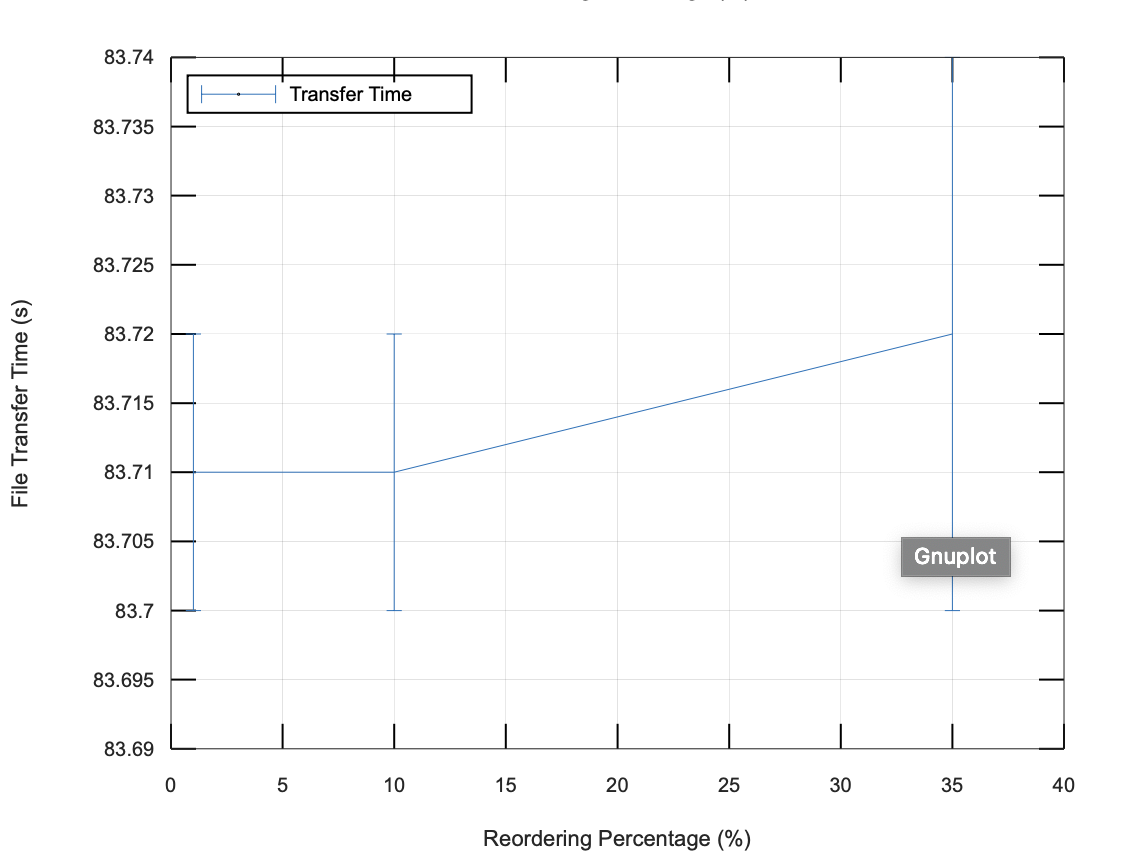
\includegraphics[scale=.45]{images/exp3.png}
    \caption{File Transfer Time(s) vs Reordering Percentage(\%)}
    \label{fig:topology}
\end{figure}
The confidence intervals are :

$ 83.7 \pm 0.01$

$83.7 \pm 0.01$

$83.71 \pm 0.02$\\
We implemented Go-Back-N mechanism to our protocol, but not same. 
In the results, we have observed that there are little changes in file transfer time for different re-ordering percentages. That might be caused because of we are starting threads separately in broker node, means either $1$ thread starts, or the other one. In theory, when re-ordering percentages changes, file transfer time should also be changes in Go-Back-N, but in our cases there is no slightly change in graph. When we add re-ordering percentage, since threads doesn't affected with them, there were no slightly changes in graph.
	
\section{Conclusion}
\label {conclusion}
In this experiment main focus is making UDP reliable (RUDP). Reliable UDP is for reliable communication. Our RUDP protocol has been implemented using one of sliding window protocols, Go-Back-N. To make our protocol reliable, we add checksum and sequence number values in the header of packet, use re-transmission and we send back Ack/nAck packets. To control the flow of transmission of data, we use flag values as condition variables. Our protocol is able to transmit large data over networks when the packet size is acceptable. As a future work, congestion control mechanism can be implemented to overcome the processing and memory overheads. Our protocol, security of the transferred data is not considered, providing it can also be done as future work. At the end, in the experiment, source and broker has TCP based connection and rest uses our protocol, we are asked to make UDP part(unreliable part) reliable, we can basically do that via TCP but this is not the problem. We have also examined our protocol versus TCP. TCP hogs all packets that are received until they came to the destination in the expecting order. This might be harmful to performance. One of the problem about TCP is about out-of-order packets. For example, in the multi-player games where only care is about the last position of player not where and what happened about a few milliseconds ago. RUDP modifications, provides most recent packet to achieve that.\\

Note that, all of the network configurations, codings, README file and report have been done by uniformly together. We worked as a pair in design, implementation, report parts and others since, composing, changing or improving any part affected the all other parts. We also use GitHub and Overleaf to make pair programming since they allow working together at the same time for people in a group.
\clearpage

\section{Appendix}
\label {appendix}
\begin{figure}[ht]
   \centering
   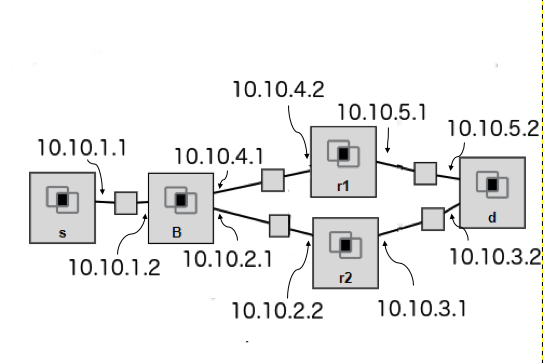
\includegraphics[scale=.40]{images/IPs.png}
    \caption{The structure of topology with IPs of interfaces}
    \label{fig:topology}
\end{figure}
\begin{figure}[ht]
   \centering
   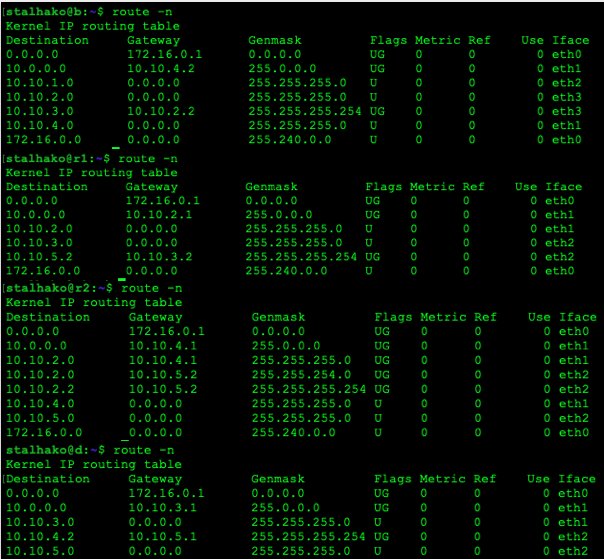
\includegraphics[scale=.40]{images/VM_default.png}
    \caption{Default Route Tables for Broker, Router1, Router 2 and Destination}
    \label{fig:topology}
\end{figure}
\newpage
\begin{figure}[ht]
   \centering
   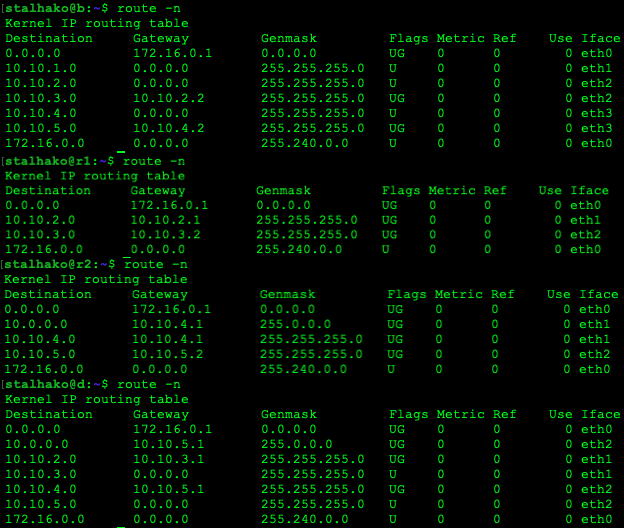
\includegraphics[scale=.40]{images/VM_after.png}
    \caption{Modified Route Tables for Broker, Router1, Router 2 and Destination}
    \label{fig:topology}
\end{figure}



\bibliographystyle{IEEEtran}
\bibliography{bibliography}

\end{document}